\documentclass{article}
\usepackage{enumitem,amssymb}
\usepackage{lipsum} % for filler text
\usepackage{fancyhdr}
\pagestyle{fancy}

\newlist{todolist}{itemize}{2}
\setlist[todolist]{label=$\square$}
\usepackage{easylist}
\usepackage{graphicx}
\fancyfoot{} % clear all footer fields
\fancyfoot[LE,RO]{\thepage}           % page number in "outer" position of footer line
\fancyfoot[RE,LO]{Version VERSIONNUMBER} % other info in "inner" position of footer line
\usepackage[margin=0.75in,headsep=.2in]{geometry}

\begin{document}
	
	{\huge \textbf{Backup a Scratch Program}}
	
\begin{enumerate}
\item {\large \textbf{Open the File Browser to "Desktop" and find your .sb3 file}}

\leftline{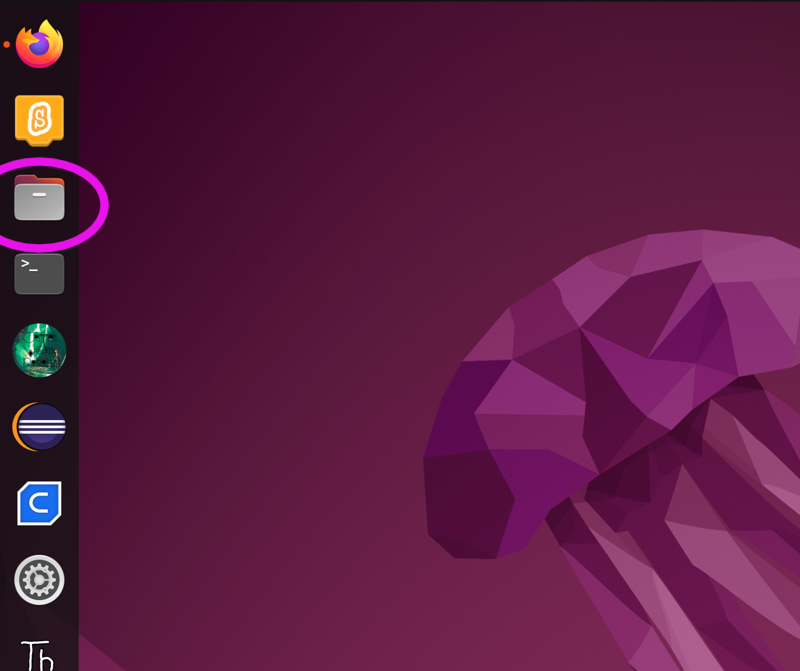
\includegraphics[scale=.15]{1.png} 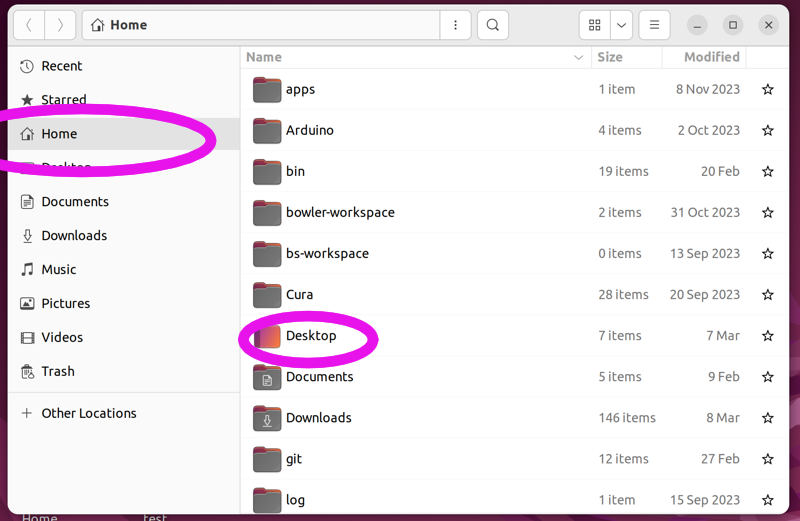
\includegraphics[scale=.20]{2.png} 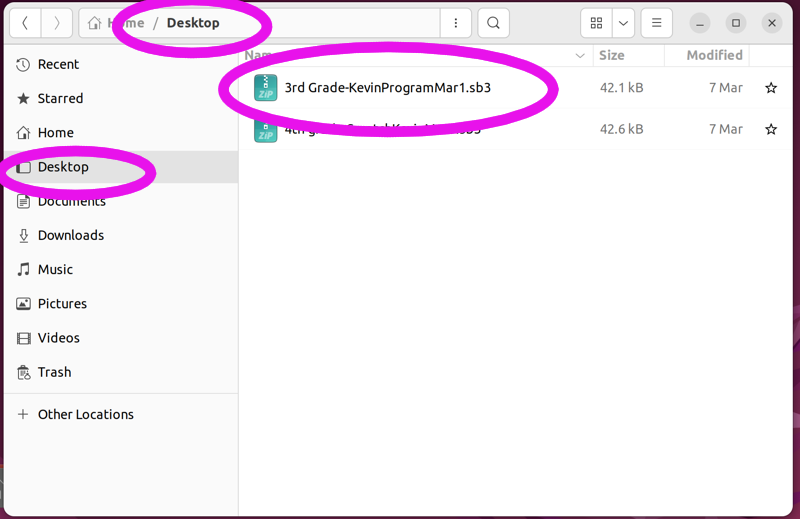
\includegraphics[scale=.20]{3.png}}

\item {\large \textbf{Re-name Your Program To Todays Date}}

\leftline{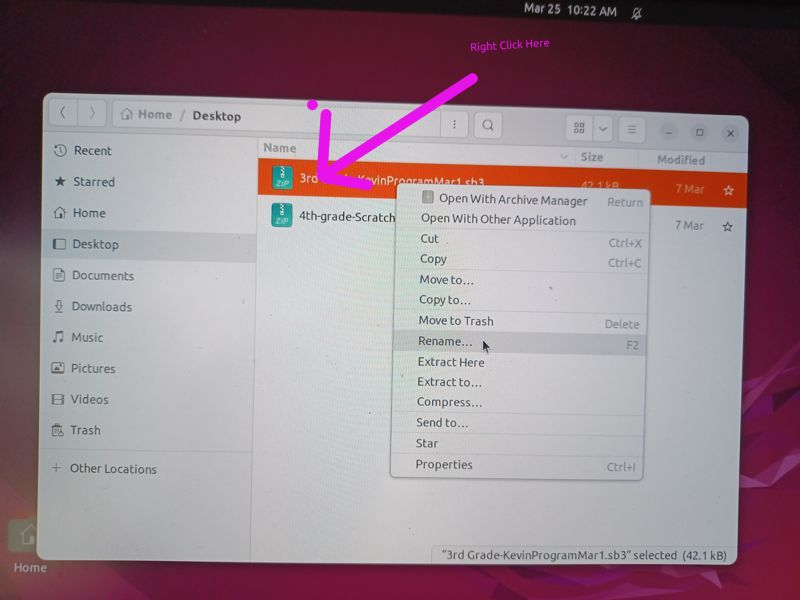
\includegraphics[scale=.30]{4.jpg} 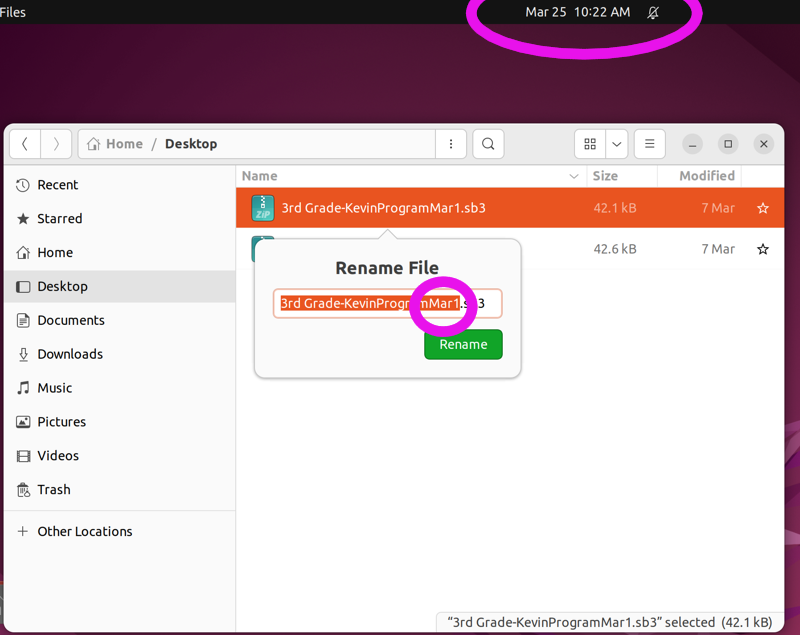
\includegraphics[scale=.30]{5.png} }

\item {\large \textbf{Open Google Drive To Your Folder}}

\leftline{ 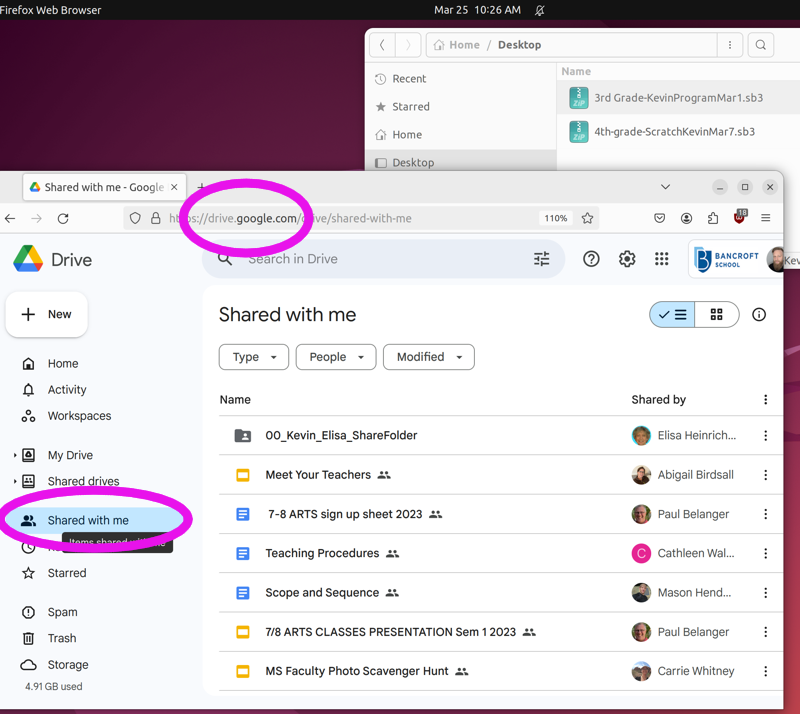
\includegraphics[scale=.20]{7.png} 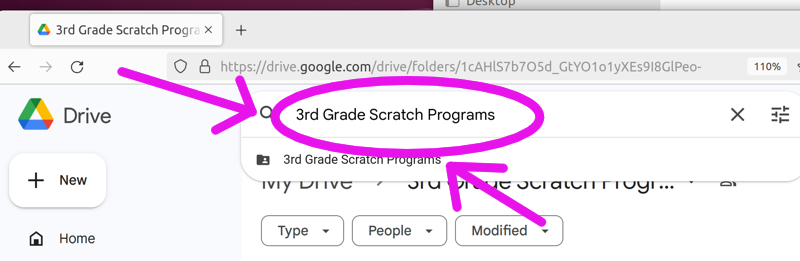
\includegraphics[scale=.25]{8.png}
	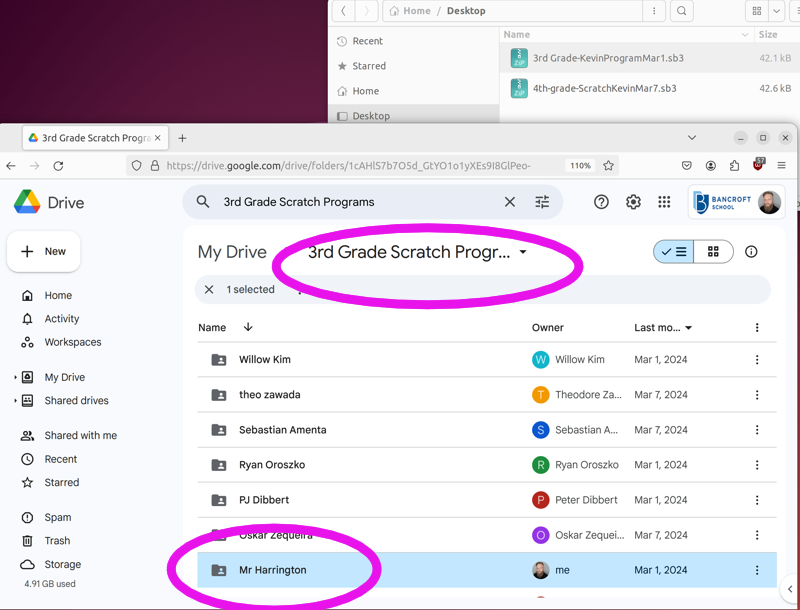
\includegraphics[scale=.20]{9.png} }


\item {\large \textbf{Upload Your Program}}

\leftline{ 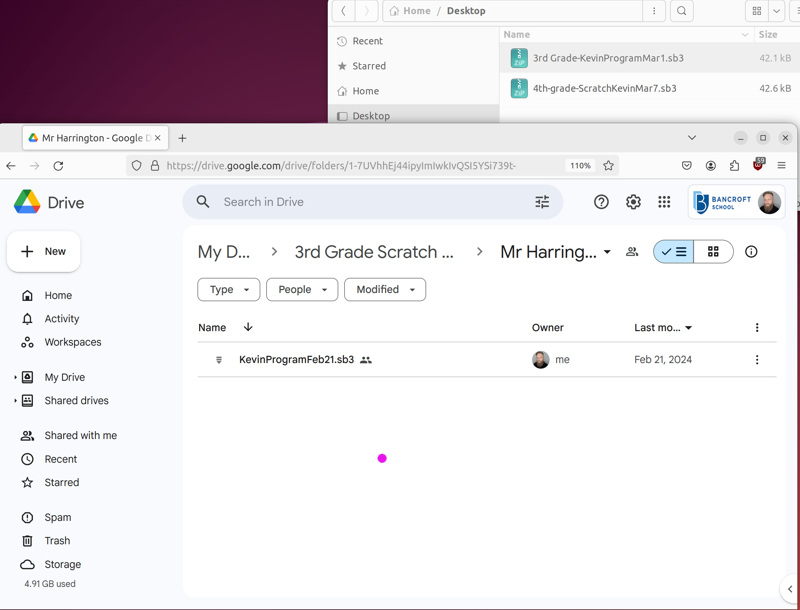
\includegraphics[scale=.20]{10.png} 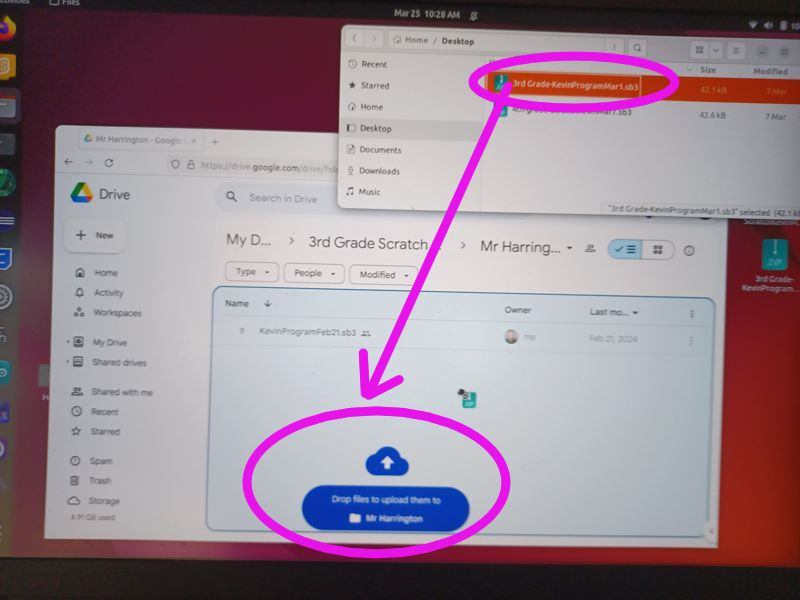
\includegraphics[scale=.20]{11.jpg}
	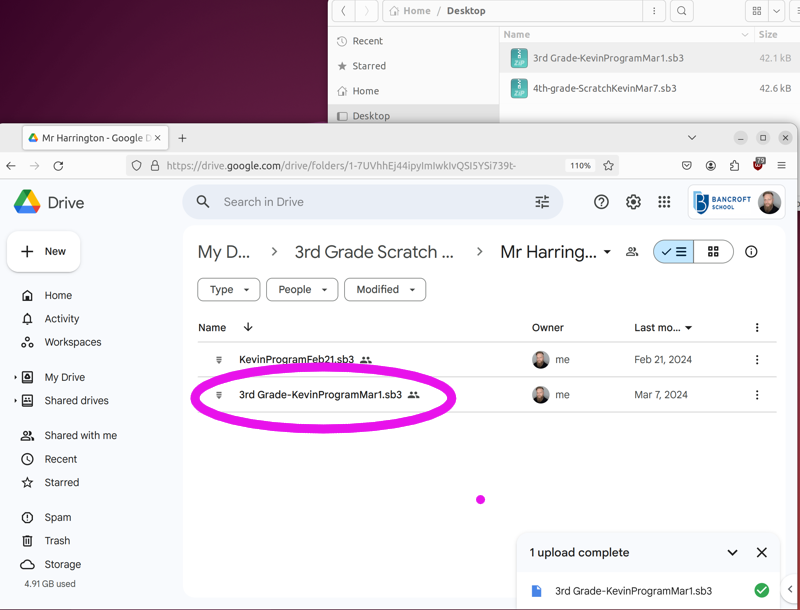
\includegraphics[scale=.20]{12.png} }
	
\end{enumerate}		

\end{document}